\documentclass[a4paper,12pt]{book}
\usepackage[margin=2cm]{geometry}		
\usepackage[latinmath,thinfonts]{uglix2}
\usepackage{array,numprint}
\usepackage{systeme}
\usepackage{multirow}
\setcounter{chapter}{8}
\begin{document}



%\iffalse %|---------------------------------

\chapter{Graphes}

\section{Introduction}
\subsection*{Plusieurs représentations}

Abel, Brieuc, Corentin, David et Ewen postent des messages sur un réseau social. Un message peut-être \og aimé\fg{} par n'importe quel utilisateur, y compris son créateur.\\
On regarde, sur une période de deux semaines, qui a aimé les messages de qui. Voici les résultats : 

\double{
\begin{enumerate}[--]
	\item 	Abel a aimé des messages de Corentin  et David;
	\item 	Brieuc a aimé ses messages et ceux de Corentin;
	\item 	Corentin a aimé les messages de David;
	\item 	David a aimé ses propres messages;
	\item 	Ewen a aimé les messages d'Abel.
\end{enumerate}
}{
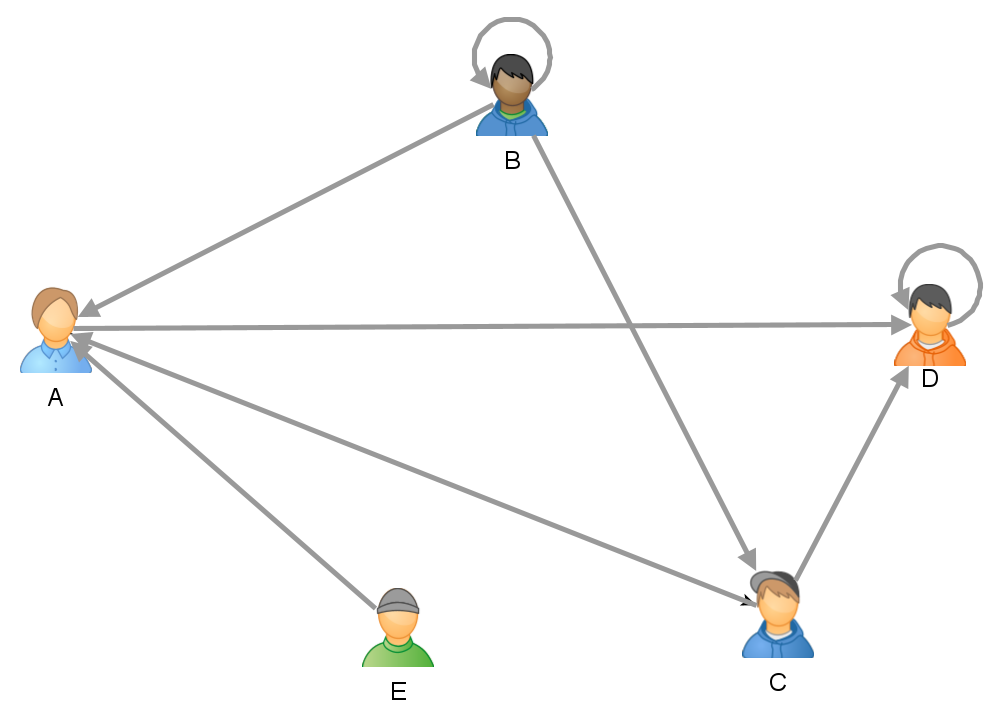
\includegraphics[width=7cm]{img/graphe1.png}}{7cm}

Ces résultats permettent de produire un \textit{graphe orienté} :
\begin{enumerate}[--]
	\item 	les \textit{sommets du graphe} représentent les personnes;
	\item 	les \textit{arêtes} sont des flèches qui représentent le fait que la personne de départ aime les messages de celle d'arrivée.
\end{enumerate}



On peut aussi représenter les résultats dans un tableau :

\begin{center}
\begin{tabular}{|l|>{\centering\arraybackslash}p{.5cm}|>{\centering\arraybackslash}p{.5cm}|>{\centering\arraybackslash}p{.5cm}|>{\centering\arraybackslash}p{.5cm}|>{\centering\arraybackslash}p{.5cm}|}
\hline
 & A & B & C & D & E \\
\hline
aime les messages de  & C,D & B,C & D & D & A \\
\hline
\end{tabular}
\end{center}

On peut aussi recopier le tableau en donnant pour chaque personne la liste de ses \og followers\fg{} (personnes qui ont aimé ses messages) :

\begin{center}
\begin{tabular}{|l|>{\centering\arraybackslash}p{1cm}|>{\centering\arraybackslash}p{1cm}|>{\centering\arraybackslash}p{1cm}|>{\centering\arraybackslash}p{1cm}|>{\centering\arraybackslash}p{1cm}|}
\hline
 & A & B & C & D & E \\
\hline
followers  & B,E & B & A,B & A,C,D & --- \\
\hline
\end{tabular}
\end{center}

On peut aussi présenter les données ainsi :

\begin{center}
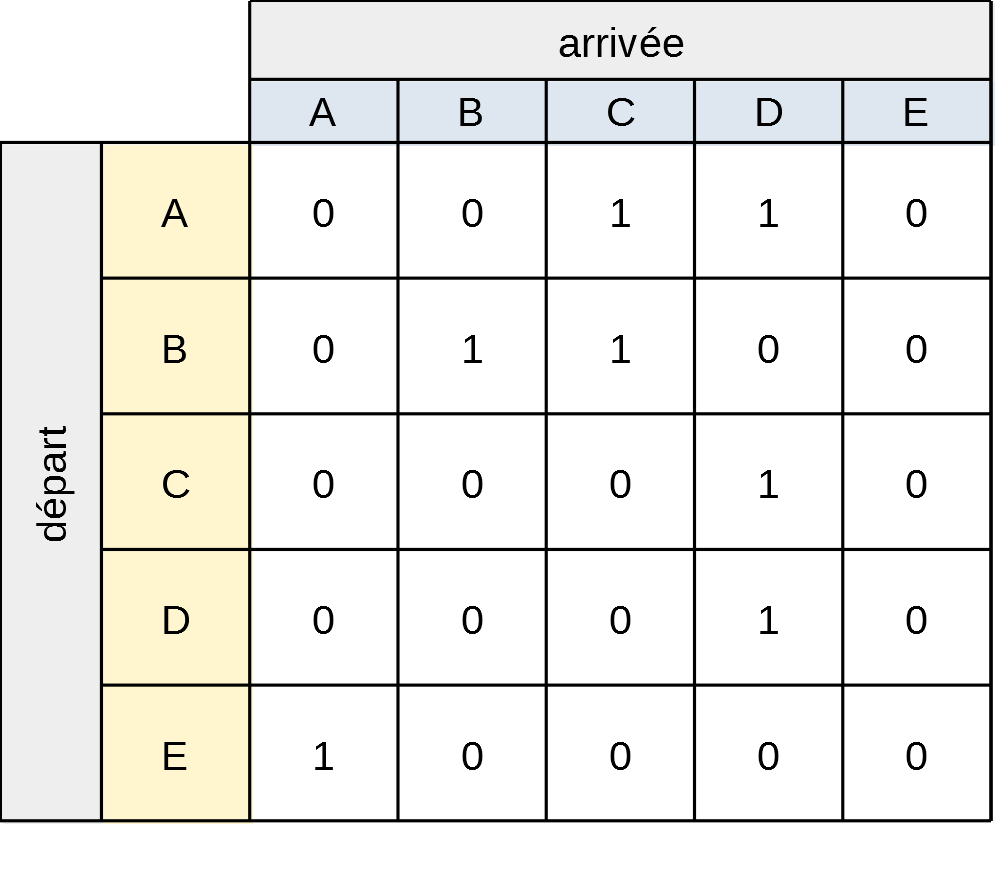
\includegraphics[width=7cm]{img/prematrice.png}
\end{center}
Il y a donc plusieurs manières de représenter un graphe orienté.

\subsection*{Organiser un graphe orienté}

On considère des individus qui ont infectés par une maladie et on place une flèche pour signifier que tel individu a contaminé tel autre individu.\\
On obtient ce résultat :
\begin{center}
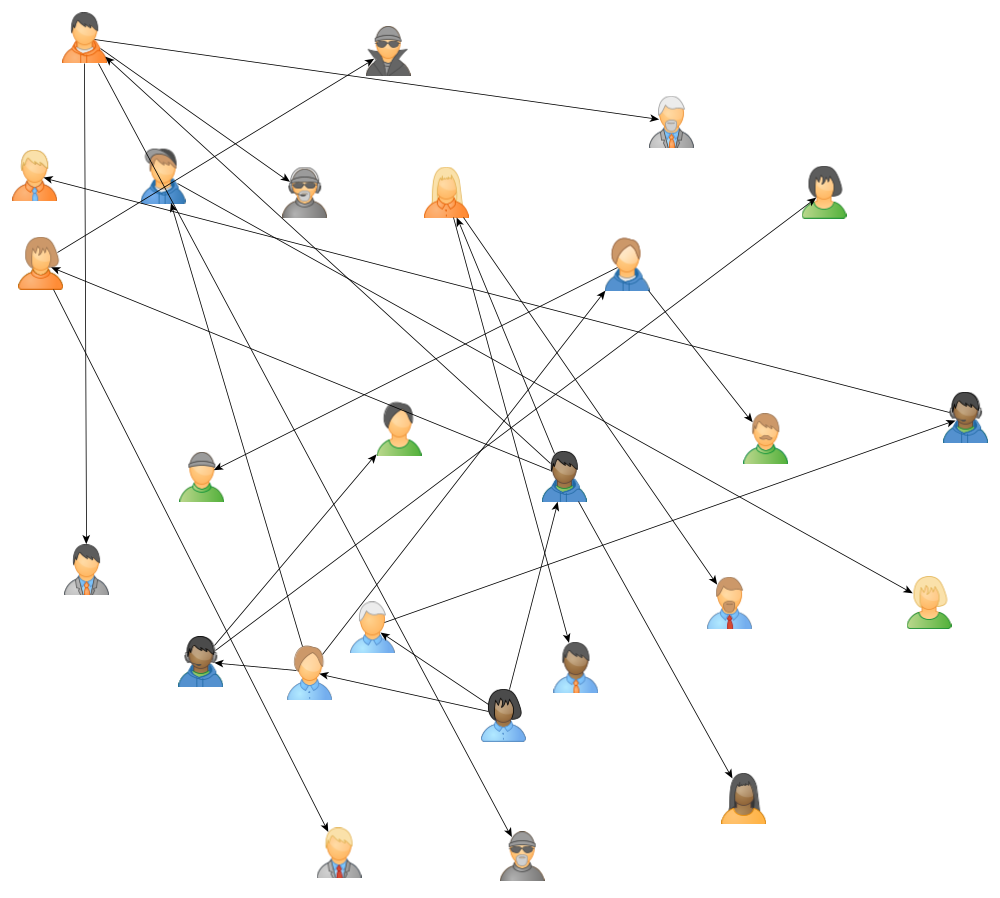
\includegraphics[width=10cm]{img/graphe2_random.png}
\end{center}
C'est le fouillis, n'est-ce pas ? \\
En déplaçant les sommets du graphe on peut le présenter ainsi :
\begin{center}
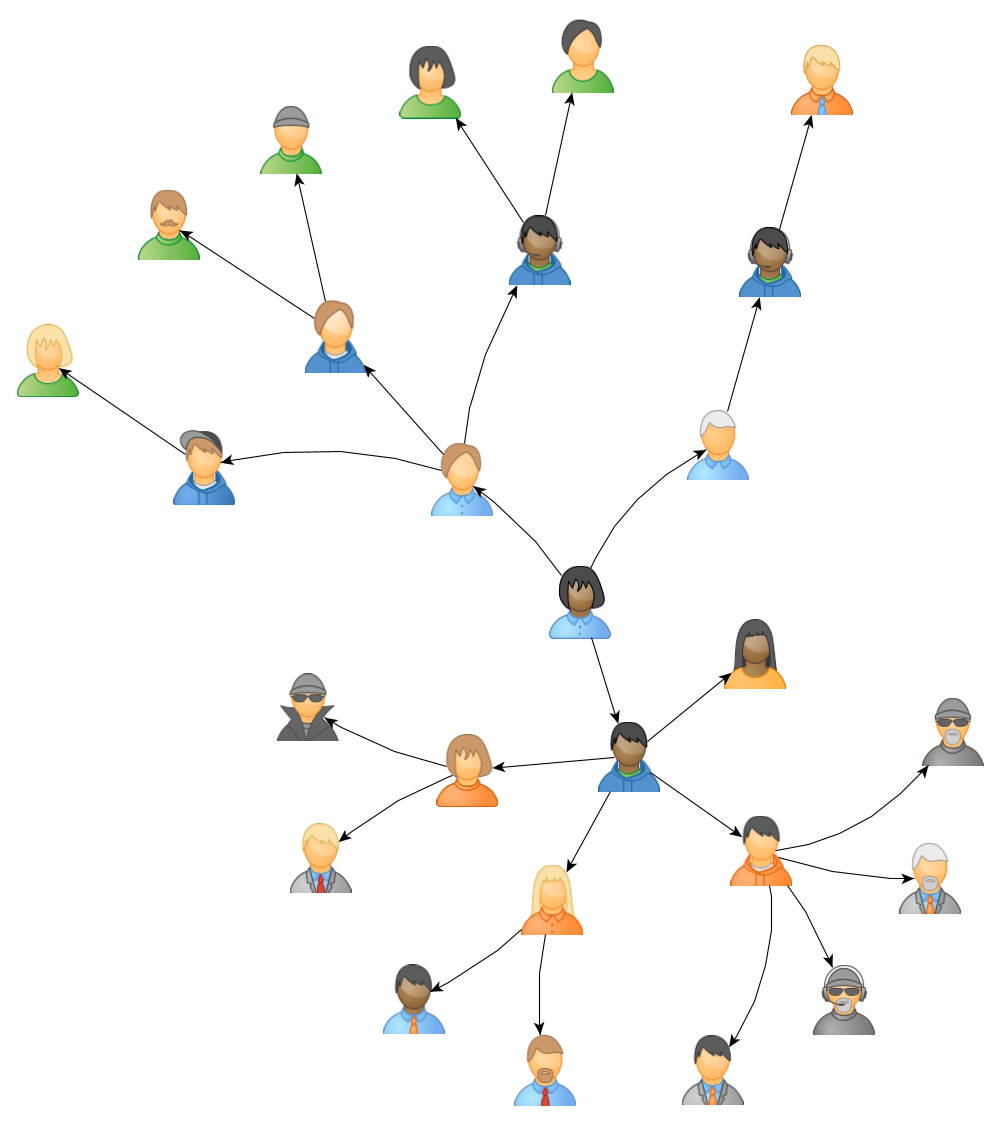
\includegraphics[width=10cm]{img/graphe2_radial.png}
\end{center}
C'est le même graphe mais on y voit plus clair... et on y voit encore plus clair comme ça :
\begin{center}
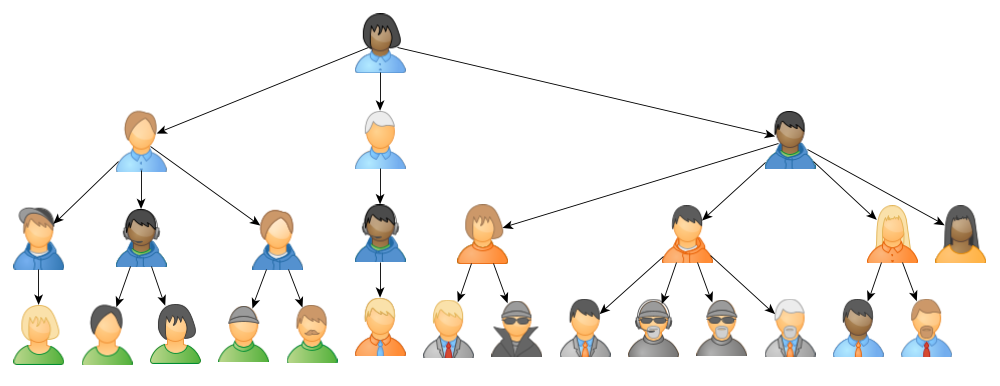
\includegraphics[width=15cm]{img/graphe2_tree.png}
\end{center}
On voit clairement le \og patient zéro\fg{}. On peut aussi rajouter des flèches quand la contamination n'est pas directe mais s'est faite \og par une ou plusieurs personnes interposées\fg{}. On obtient ceci
\begin{center}
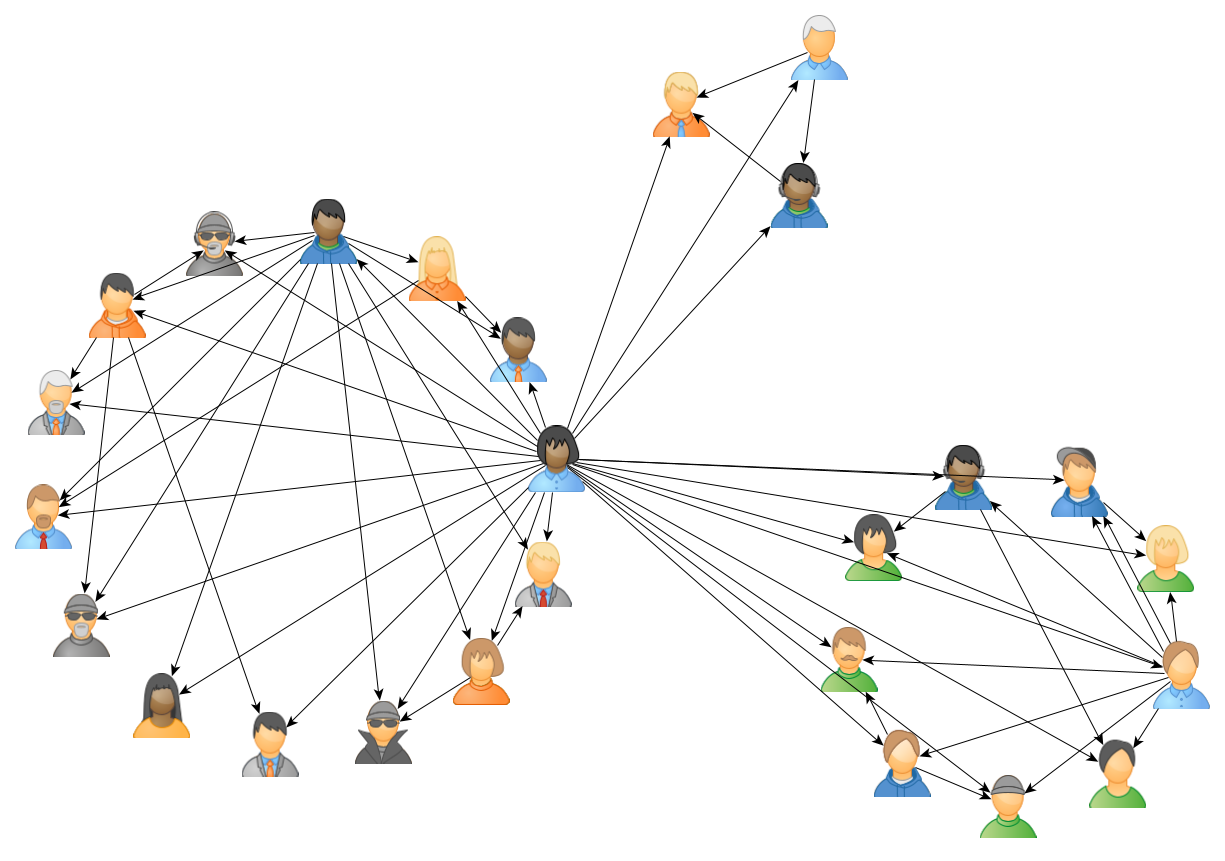
\includegraphics[width=13cm]{img/graphe2_transitif.png}
\end{center}

Le but de ce chapitre est de formaliser tout cela (et plus).

\section{Représentations d'un graphe orienté}
\subsection{Premières notions}
\begin{definition}[ : graphe, sommet, arc]
Un graphe orienté, c'est la donnée de
\begin{enumerate}[--]
	\item 	un ensemble $S=\{s_1;\,...;\,s_n\}$ de \textit{sommets};
	\item 	un ensemble $A$ composé d'\textit{arcs} du type $(s_i;\,s_j)$, qui indiquent qu'il y a \og une flèche\fg{} partant du sommet $s_i$ et allant au sommet $s_j$.:\\ $s_i$ est appelé l'\textit{origine} de l'arc et $s_j$ son \textit{extrémité}.
\end{enumerate}
\end{definition}

\begin{exemple}[]
\double{Ici l'ensemble des sommets est $\{A;\,B;\,C;\,D\}$.\\
L'ensemble des arcs est :\\
$\{(A;B);\,(B;A);\,(B;C);\,(B;D);\,(C;D)\}$}{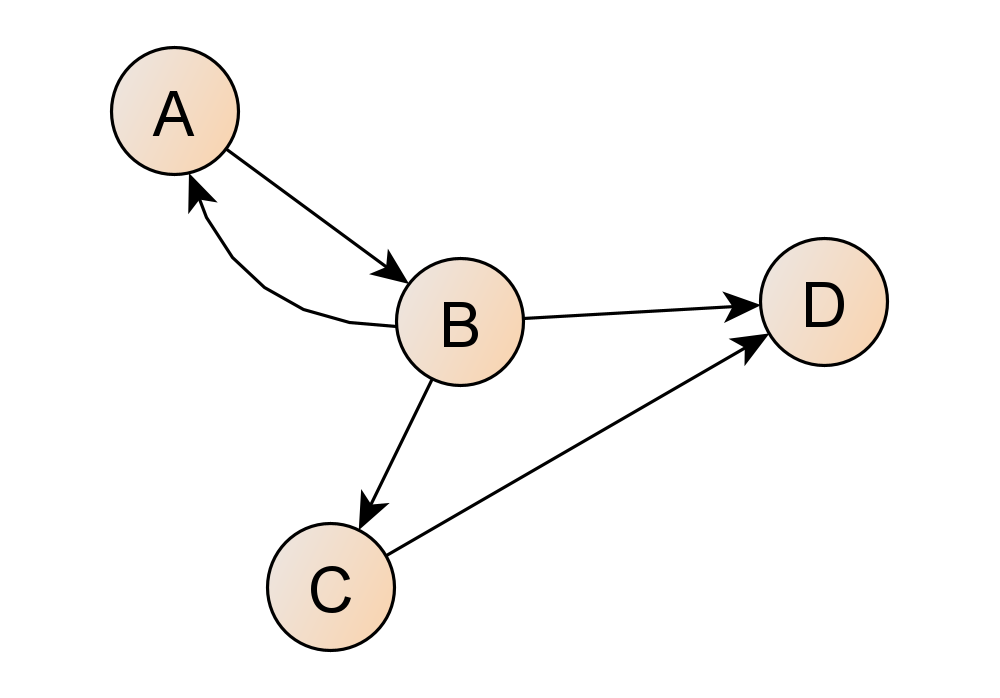
\includegraphics[width=7cm]{img/ex_graphe_oriente.png}}{7cm}
\end{exemple}

\begin{exercice}[]
Donner l'ensemble des sommets et l'ensemble des arêtes du graphe suivant.
\begin{center}
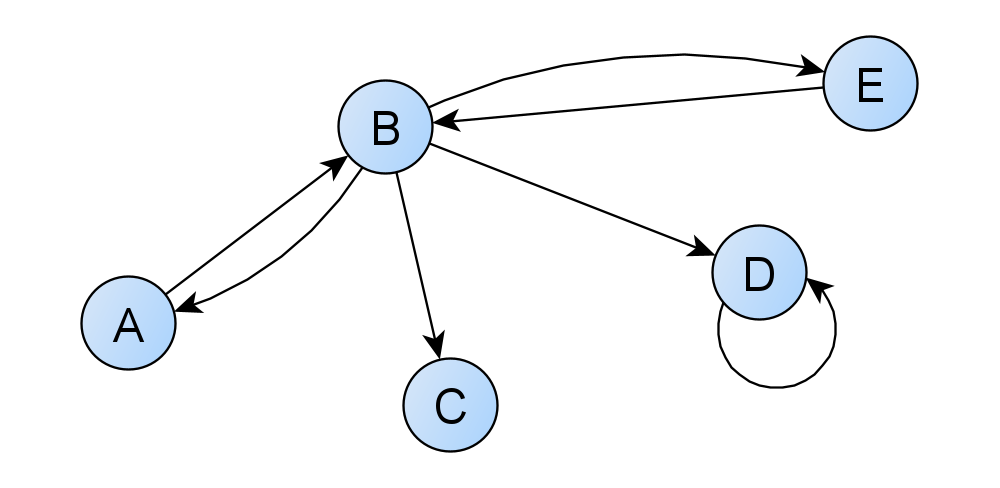
\includegraphics[width=7cm]{img/exo_graphe.png}
\end{center}
\end{exercice}
\begin{definition}[ : boucle]
Un arc dont l'origine et l'extrémité sont confondues d'appelle une \textit{boucle}.
\end{definition}
\subsection{Successeurs, prédécesseurs}

\begin{definition}[ : successeur, prédécesseur]
Soit un graphe de sommets $S$ et d'arcs $A$. Soit $s$ un sommet.\\
On note $\Gamma^+(s)$ l'ensemble des \textit{successeurs de $s$}.\\
C'est l'ensemble des extrémités des arcs \textit{partant de} $s$.\\
De même, on note $\Gamma^-(s)$ l'ensemble des \textit{prédécesseurs de $s$}.\\
C'est l'ensemble des origines des arcs \textit{arrivant sur} $s$.\\
\end{definition}


\begin{exemple}[s]
\double{Dans ce graphe, il y a 4 arcs d'origine D. Leurs extrémités sont les points C,D,E et F.\\ Ainsi $\Gamma^+(D)=\{C;\,D;\,E;\,F\}$.}{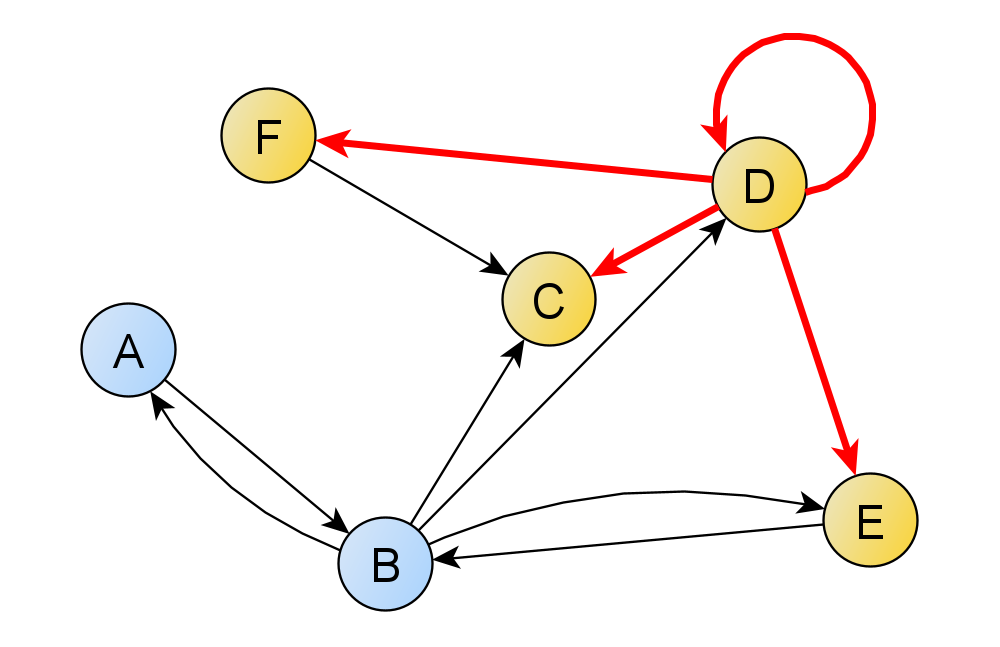
\includegraphics[width=7cm]{img/successeurs.png}}{7cm}

On peut retrouver le graphe à partir du tableau des successeurs.

\begin{center}
\begin{tabular}{|c|c|c|c|c|c|c|}
\hline
sommet & A & B & C & D & E & F \\
\hline
successeurs & B & A, C, E & --- & C, D, E, F & B & C \\
\hline
\end{tabular}
\end{center}

\double{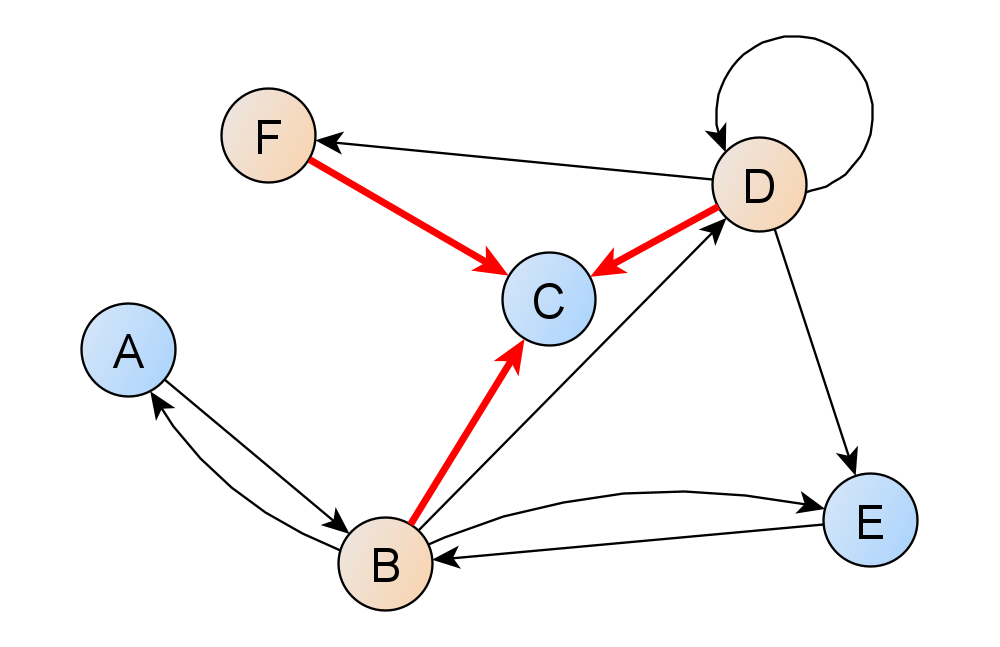
\includegraphics[width=7cm]{img/predecesseurs.png}}{Dans ce graphe, il y a 3 arcs d'extrémité C.\\ 
Leurs origines sont les points B,D et F.\\ Ainsi $\Gamma^-(C)=\{B;\,D;\,F\}$.}{9.7cm}
On peut retrouver le graphe à partir du tableau des prédécesseurs.

\begin{center}
\begin{tabular}[color=white]{|c|c|c|c|c|c|c|}
\hline
sommet & A & B & C & D & E & F \\
\hline
prédécesseurs & B & A, E & B, D, F & B, D & B, D & D \\
\hline
\end{tabular}
\end{center}
\end{exemple}

\begin{exercice}[]
Pour chacun des graphes, donne le tableau des successeurs et celui des prédécesseurs (attention : pour le graphe de gauche, on a dessiné des arcs bidirectionnels, chacun compte pour 2 arcs).
\begin{center}
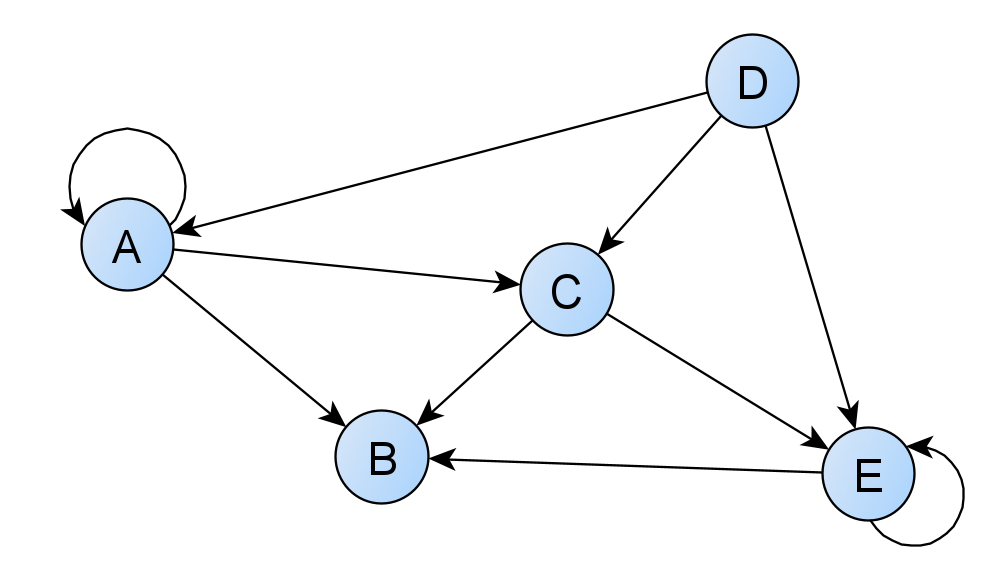
\includegraphics[width=7cm]{img/exo1_graphe1.png}\hspace*{2cm}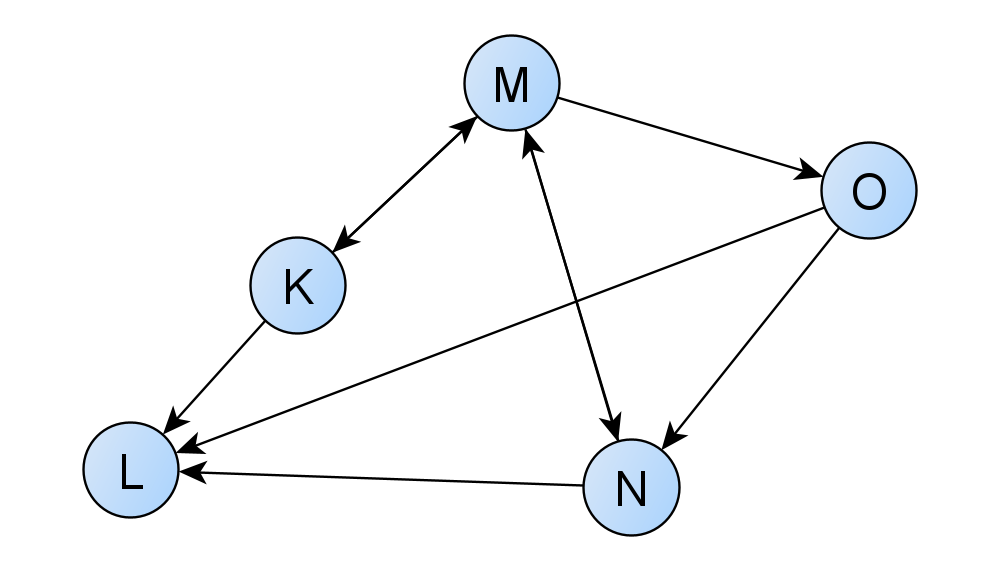
\includegraphics[width=7cm]{img/exo1_graphe2.png}
\end{center}
\end{exercice}


\begin{exercice}[]
Dessine le graphe correspondant au tableau de successeurs.
\begin{center}
\begin{tabular}{|c|c|c|c|c|}
\hline
sommet 		& A		 & B 		& C		 & D \\
\hline
successeurs & A,B,C 	& B,C,D 	& C,D,A 		& D,A,B\\
\hline
\end{tabular}
\end{center}
\end{exercice}


\begin{exercice}[]
Dessine le graphe correspondant au tableau de prédécesseurs.
\begin{center}
\begin{tabular}{|c|c|c|c|c|c|}
\hline
sommet 		& A		 & B 		& C		 & D \\
\hline
prédécesseurs & A,D 	& --- 	& A,B,D 		& A\\
\hline
\end{tabular}
\end{center}
\end{exercice}

\subsection{Matrice d'adjacence}

\begin{definition}[ : matrice d'adjacence]

Soit un graphe G de sommets  $S=\{s_1;\,...;\,s_n\}$ et d'arcs A. On appelle \textit{matrice d'adjacence de} G la matrice carrée d'ordre n $M=(m_{ij})$ telle que 
\begin{enumerate}[--]
	\item 	$m_{ij}=1$ s'il y a un arc partant de $s_i$ et arrivant sur $s_j$;
	\item 	$m_{ij}=0$ sinon.
\end{enumerate}
\end{definition}

\begin{exemple}[]
\ \\[-.2em]
\double{En écrivant les sommets dans l'ordre alphabétique, la matrice d'adjacence du graphe ci-contre est

$$ M=\begin{pmatrix}
1 &1 &0 & 0&0  \\
0 & 0&1 &0 &0  \\
0 & \boxed{1} & 0 & 0 & 1\\
1 & 0 & 1 & 0 & 1\\
0 & 1 & 0 &{\color{red}1} & 0 
\end{pmatrix}$$
}
{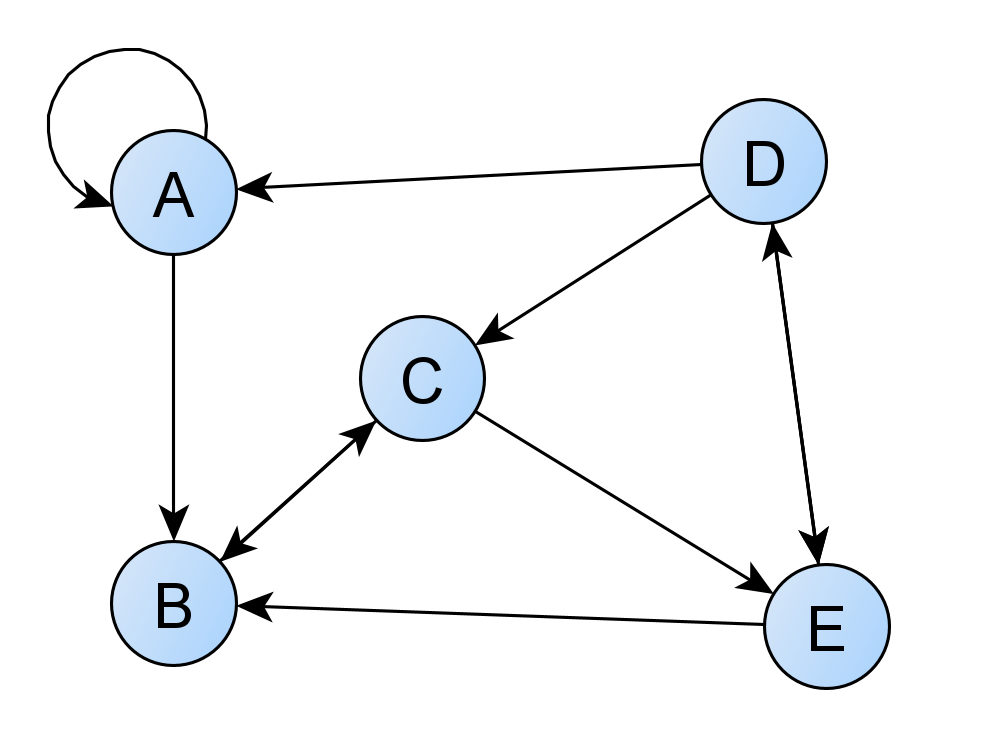
\includegraphics[width=7cm]{img/matr_adj1.png}}{7cm}

L'élément encadré de M est à la 3\eme ligne et à la 2\eme colonne : c'est $m32$. Il vaut 1 et signifie qu'il y a un arc partant du sommet 3, donc C, et allant au sommet 2, donc B.\\
De même, du 5\eme sommet E, il existe un arc allant vers le 4\eme (D), donc $m_{54}=1$ (en rouge).
\end{exemple}

\begin{remarque}[]
Dans une matrice d'adjacence\begin{enumerate}[--]
	\item 	Les lignes correspondent au points de départ, les colonnes au point d'arrivée;
	\item 	Sur une ligne donnée(la i\eme par exemple), on peut lire \textit{tous les successeurs} de $s_i$;
	\item 	Sur une colonne donnée, (la j\eme par exemple), on lite \textit{tous les prédécesseurs} de $s_j$;
\end{enumerate}
\end{remarque}

\begin{exercice}[]
On considère un graphe dont l'ensemble des sommets est $\{A;\,B;\,C;\,D;\,E;\,F\}$, et dont la matrice d'adjacence est
$$ M=\begin{pmatrix}
1 &1 &0 & 1&0&1  \\
0 & 0&0 &1 &0&1  \\
1 & 0 & 0 & 0 & 1&1\\
1 & 0 & 1 & 1 & 1&0\\
0 & 1 & 0 &1 & 1 &1\\
1 & 0 &1 & 0 &1& 0
\end{pmatrix}$$

\begin{enumerate}[\bfseries 1.]
	\item 	Donner le tableau des successeurs de chaque sommet.
	\item 	Donner le tableau des prédécesseurs de chaque sommet.
	\item 	Représenter ce graphe.
\end{enumerate}
\end{exercice}

\section{Chemins et circuits}

\begin{definition}[s : chemin, longueur]

On considère un graphe orienté.\\
Un \textit{chemin} est une succession de sommets dans un ordre donné, chacun étant relié au suivant par un arc.\\
La \textit{longueur} du chemin, c'est le nombre d'arcs qui composent le chemin. C'est aussi le nombre de sommets qui composent le chemin mois un.
\end{definition}

\begin{exemple}[]
\double{$(F,\,C,\,D,\,E)$ est un chemin de longueur 3.\\
$(F,\,C,\,B,\,E)$ n'en est pas un car l'arc $(C,\,B)$ n'existe pas. }{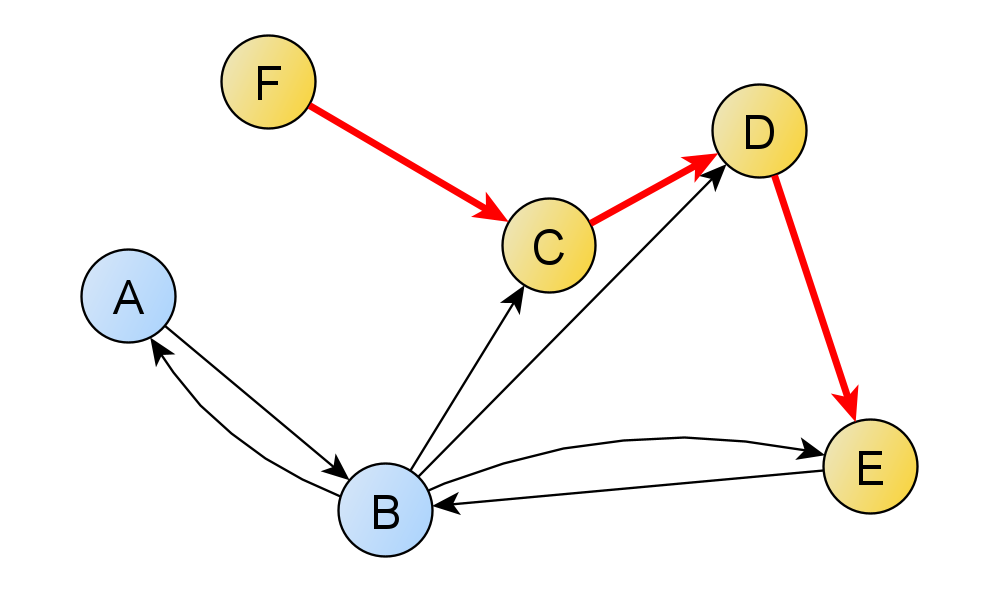
\includegraphics[width=7cm]{img/chemin.png}}{7cm}
\end{exemple}

\begin{definition}[s : chemin hamiltonien,circuit]

Un \textit{chemin hamiltonien} est un chemin qui passe une et une seule fois par \textit{chaque} sommet.\\
Un \textit{circuit} est un chemin dont le premier et le dernier sommet sont identiques (un chemin \og fermé\fg{} en quelque sorte).
\end{definition}


\begin{exemple}[s]

\double{$(C,\,D,\,E,\,B,\,C)$ est un circuit de longueur 4.}{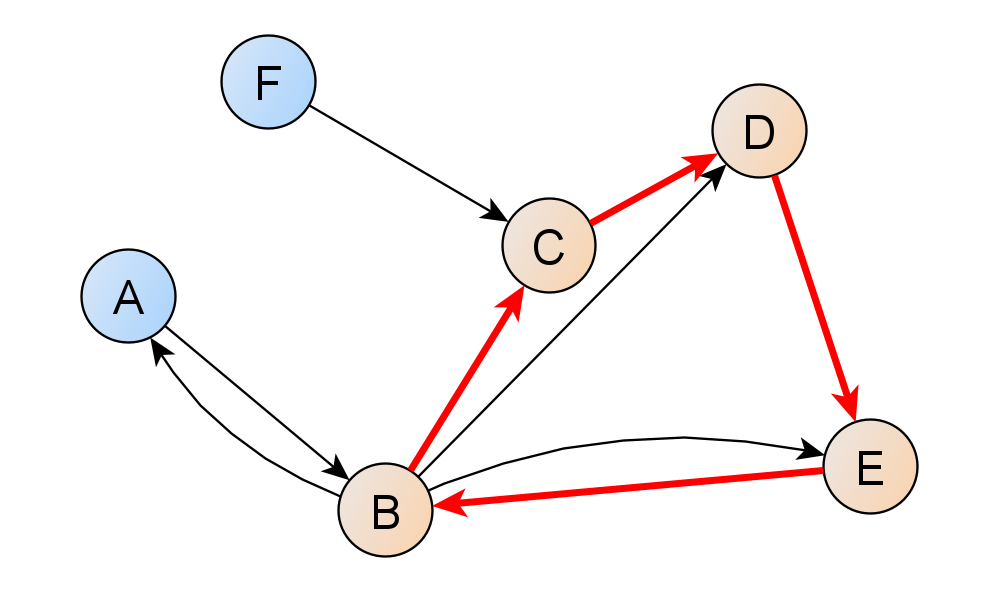
\includegraphics[width=7cm]{img/circuit.png}}{7cm}\\

\double{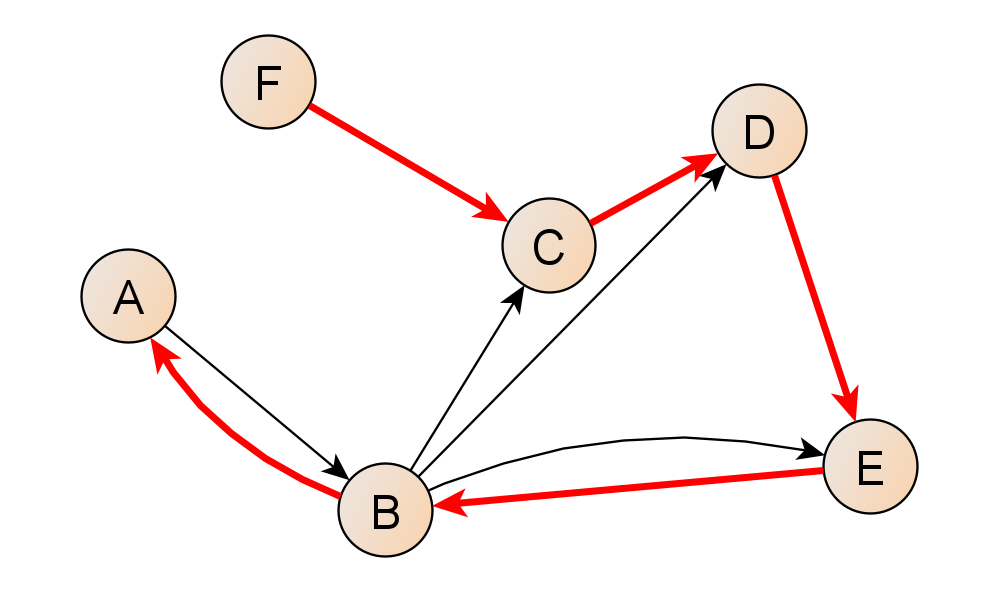
\includegraphics[width=7cm]{img/chemin_hamiltonien.png}}{$(F,\,C,\,D,\,E,\,B,\,A)$ est un chemin hamiltonien.}{9cm}\\

\end{exemple}

\begin{remarque}[]
Un graphe orienté \textit{ne possède pas toujours} de circuit hamiltonien (à gauche) ou bien peut en posséder plusieurs (à droite).
\begin{center}
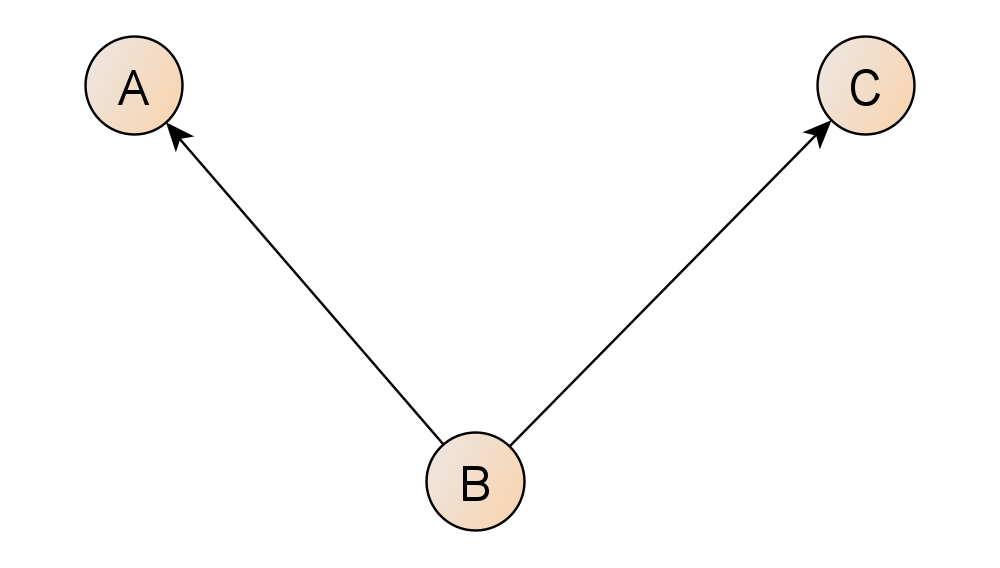
\includegraphics[width=7cm]{img/pas_de_ch.png}\hspace{2cm}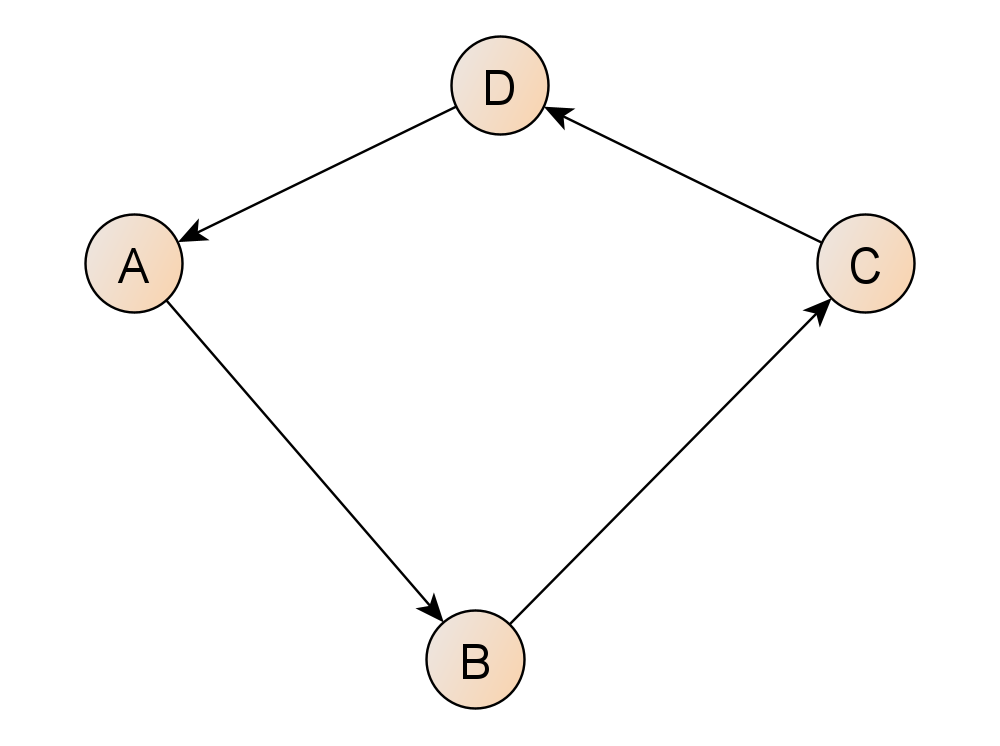
\includegraphics[width=7cm]{img/plusieurs_ch.png}
\end{center}
\end{remarque}

\begin{exercice}[]
Trouve un chemin hamiltonien, un circuit de longueur 3 et un autre de longueur 4.
\begin{center}
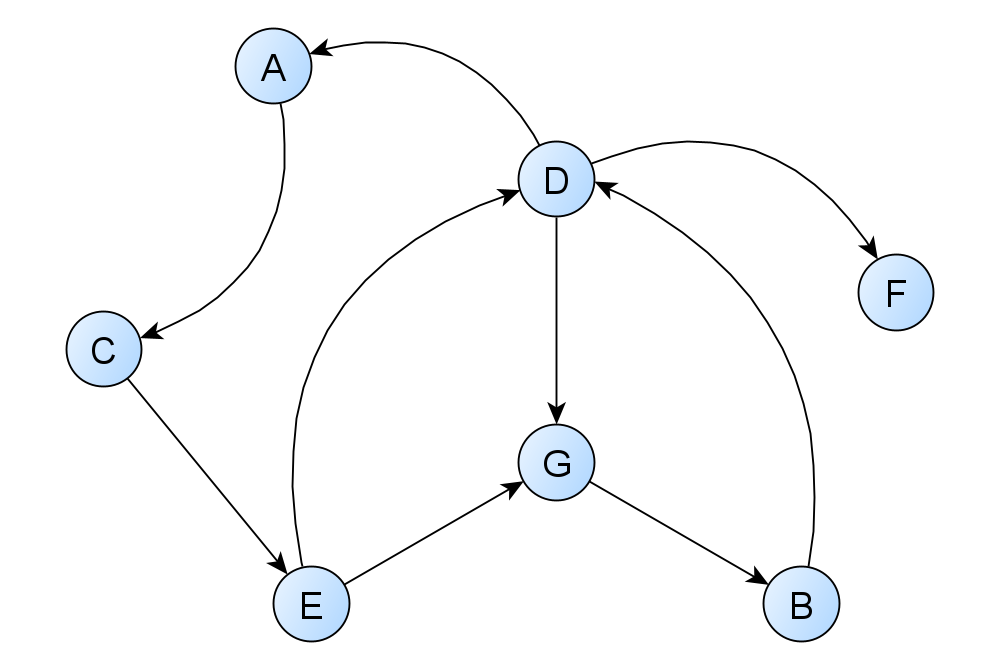
\includegraphics[width=7cm]{img/ex_circuit_ch.png}
\end{center}
\end{exercice}

\section{Utilité des matrices d'adjacence}
On peut se poser beaucoup de questions ayant trait aux chemins d'un graphe. En voici trois que nous allons étudier :
\begin{enumerate}[--]
	\item 	On se donne un graphe à 10 sommets, on en choisit un en particulier. Combien de chemins différents de longueur 5 commencent en ce sommet ?
	\item 	Toujours dans ce graphe, combien y a-t-il de chemin de longueur 5 ?
	\item 	Si on veut (comme dans l'exemple introductif) ajouter tous les \og raccourcis\fg{} aux arcs du graphe, comment s'y prendre pour n'en oublier aucun ?
\end{enumerate}



\begin{propriete}[]
Soit $G$ un graphe possédant $n$ sommets $s_1$, $s_2$, \ldots $s_n$ et $M$ sa matrice d'adjacence.\\
Soit $p$ un entier naturel positif. Alors $M^p$ contient les informations sur les chemins de longueur $p$ du graphe :

Le nombre de chemins de longueur $p$ reliant $s_i$ à $s_j$ est le coefficient de la i\eme ligne et de la j\eme colonne de $M^p$.
\end{propriete}

\begin{exemple}[]
\double{La matrice d'adjacence du graphe ci-contre est 
$$M=\begin{pmatrix}
0 & 1 & 0 & 0 & 1\\
0 & 0 & 1 & 0 & 1\\
0 & 0 & 0 & 1 & 0\\
0 & 0 & 0 & 0 & 0\\
0 & 0 & 0 & 1 & 0
\end{pmatrix}$$
Pour déterminer les chemins de longueur 3, calculons $M^3$ \textit{à l'aide de la calculatrice} :
}{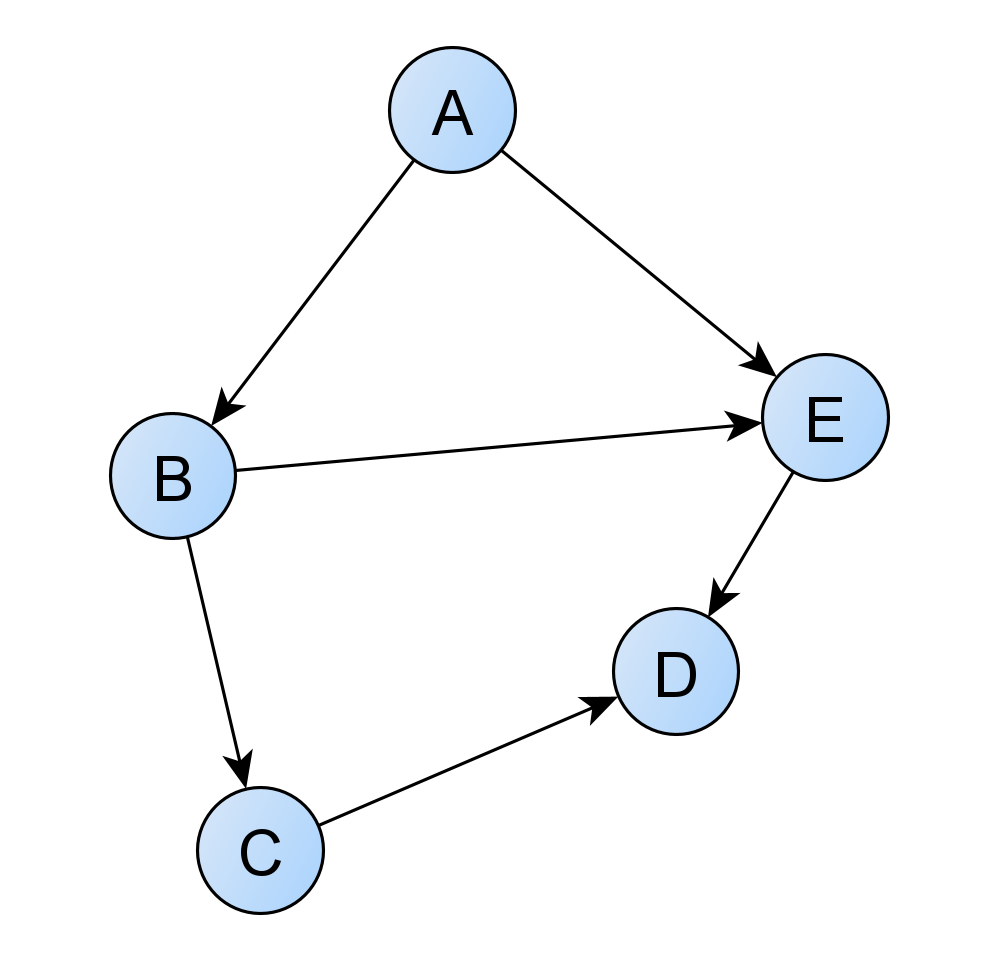
\includegraphics[width=7cm]{img/exemple_Mp.png}}{7cm}

$M^3 = \begin{pmatrix}
0 & 0 & 0 & 2 & 0\\
0 & 0 & 0 & 0 & 0\\
0 & 0 & 0 & 0 & 0\\
0 & 0 & 0 & 0 & 0\\
0 & 0 & 0 & 0 & 0\\
\end{pmatrix}$ et seul coefficient non nul est à la 1\ere ligne (départ A) et à la 3\eme colonne (arrivée D): il n'y a que 2 chemins de longueur 3 dans ce graphe, et ils relient $A$ à $D$.\\
Maintenant qu'on connaît leur nombre et leurs extrémités, on peut les écrire : $(A,\,B,\,E,\,D)$ et $(A,\,B,\,C,\,D)$.
\end{exemple}

\begin{remarque}[]
Ce procédé ne donne pas la liste des chemins de longueur donnée, seulement leur nombre et leurs extrémités.
\end{remarque}

\begin{exercice}[]
On donne le tableau de prédécesseurs suivants :
\begin{center}
\begin{tabular}{|l|>{\centering\arraybackslash}p{1cm}|>{\centering\arraybackslash}p{1cm}|>{\centering\arraybackslash}p{1cm}|>{\centering\arraybackslash}p{1cm}|>{\centering\arraybackslash}p{1cm}|>{\centering\arraybackslash}p{1cm}|}
\hline
sommet		 	& A 	& B 	& C 	& D 	& E 	& F\\
\hline
prédécesseurs 	& --- 	& --- 	& A,B,E & F 	& B,D   & A,B\\
\hline
\end{tabular}
\end{center}
En utilisant les puissances de la matrice d'adjacence :
\begin{enumerate}[--]
	\item 	Donner tous les chemins de longueur 3.
	\item 	Montrer qu'il n'existe pas de chemin de longueur 4.
	\item 	Montrer que ce graphe ne possède pas de circuit.
\end{enumerate}
\end{exercice}

\section{Matrices booléennes et fermeture transitive}


Parfois on n'a pas besoin de connaître le nombre précis de chemins d'une longueur donnée reliant deux sommets. On veut juste savoir s'il en existe au moins un ou pas. Les matrices booléennes vont nous permettre de répondre simplement à cette question.\\


La matrice d'adjacence d'un graphe ne comporte que des zéros et des uns donc on peut la voir comme une \textit{matrice booléenne}, c'est à dire une matrice à coefficients dans l'algèbre de Boole $\mathcal{B}=\left\{ 0;\,1\right\}$. Pour rappel, cette algèbre de Boole est munie des opérations binaires $+$ et $\times$ vérifiant :
\begin{enumerate}[\textbullet]
	\item 	$0+0 = 0$, $1+0 = 1$ et $1+1 = 1$ (penser au \og ou\fg{} logique)
	\item 	$0\times 0=0$, $1\times 0=0$ et $1\times 1 = 1$ (penser au \og et\fg{} logique)
\end{enumerate}

\begin{definition}[s : addition et multiplication de matrices booléennes]
Soient $A$ et $B$ 2 matrices booléennes.
\begin{enumerate}[--]
	\item 	On définit $A\oplus B$, somme \textit{booléenne} de $A$ et de $B$ comme ceci : chaque coefficient de $A\oplus B$ est la somme booléenne des coefficients correspondants de $A$ et de $B$.\\
	En pratique on calcule $A+B$ comme d'habitude et on remplace chaque coefficient non nul par un 1.
	\item 	On définit $A\otimes B$, produit \textit{booléenne} de $A$ et de $B$ comme suit : on calcule $A\times B$ comme d'habitude et on remplace chaque coefficient non nul par un 1.
\end{enumerate}
\end{definition}
\begin{exemple}[s]

Prenons $A=\begin{pmatrix}
1 & 1 & 1 \\
0 & 0 & 1 \\
1 & 0 & 1 \\
\end{pmatrix}$ et $B=\begin{pmatrix}
0 & 1 & 0 \\
1 & 0 & 1 \\
1 & 0 & 1 \\
\end{pmatrix}$.
\begin{enumerate}[\textbullet]
	\item 	$A+B=\begin{pmatrix}
	1 & 2 & 1 \\
	1 & 0 & 2 \\
	2 & 0 & 2 \\
	\end{pmatrix}$ donc $A\oplus B=\begin{pmatrix}
		1 & 1 & 1 \\
		1 & 0 & 1 \\
		1 & 0 & 1 \\
		\end{pmatrix}$
	\item 	$A\times B =\begin{pmatrix}
		2 & 1 & 2 \\
		1 & 0 & 1 \\
		1 & 1 & 1 \\
		\end{pmatrix}$ donc $A\otimes B=\begin{pmatrix}
			1 & 1 & 1 \\
			1 & 0 & 1 \\
			1 & 1 & 1 \\
			\end{pmatrix}$
\end{enumerate}
\end{exemple}

\begin{definition}[ : puissance d'une matrice booléenne]

Soit $A$ une matrice booléenne carrée de taille $n$.\\
On pose $A^{[O]}=I_n$, $A^{[1]}=A$ et pour tout entier $p$ supérieur à 1:
$$A^{[p]}=\underbrace{A\otimes\ldots \otimes A}_{p\text{\ facteurs}}$$
En pratique il suffit de calculer $A^p$ et de remplacer les coefficients non nuls par des 1.
\end{definition}

\begin{exemple}[]
Prenons $A =\begin{pmatrix}
0 & 1 & 0\\1&0&1\\1&1&0
\end{pmatrix}$ et $p=3$.\\
Avec la calculatrice on obtient $A^3 =\begin{pmatrix}
1 & 2 & 0\\2&1&2\\2&2&1
\end{pmatrix}$ donc $A^{[3]} =\begin{pmatrix}
1 & 1 & 0\\1&1&1\\1&1&1
\end{pmatrix}$.\\

Si $A$ est la matrice d'adjacence d'un graphe alors $A^{[3]}$ nous indique si 2 sommets du graphe peuvent être reliés ou non par un chemin de longueur 3 : on voit que c'est toujours possible sauf pour relier le 1\er au 3\eme.
\end{exemple}
%\fi %---------------------------------------


On considère un graphe et on veut (comme dans l'exemple introductif) ajouter tous les \og raccourcis\fg{} aux arcs du graphe, comment s'y prendre pour n'en oublier aucun ?

Si notre graphe possède $n$ sommets, considérons 2 sommets $s_i$ et $s_j$, on veut rajouter l'arc $(s_i,\, s_j)$ (qu'on va appeler \textit{raccourci}) aux arcs du graphe dès qu'il existe un chemin allant de $s_i$ à $s_j$.\\
Nous allons admettre que c'est le cas si (et seulement si) il existe un chemin de longueur 1, ou 2, ..., ou $n-1$ qui relie ces 2 sommets. On arrive alors à la propriété et définition suivante :

\begin{propriete}[ et définition]
Soit $M$ la matrice d'adjacence d'un graphe $G$ à $n$ sommets. On définit
$$\widehat{M}=M\oplus M^{[2]}\oplus\ldots\oplus M^{[n-1]}$$

$\widehat{M}$ est la matrice d'adjacence du graphe appelé \textit{fermeture transitive} de $G$, composé des mêmes sommets et arcs que ceux de $G$, auxquels on ajoute tous les arcs des \og raccourcis\fg{}.
\end{propriete}

\begin{methode}[ : déterminer une fermeture transitive]
\double{On se donne le graphe ci-contre, dont la matrice d'adjacence est

$$M=\begin{pmatrix}0&0&1&1\\0&0&0&1\\0&1&0&0\\0&0&0&0\end{pmatrix}$$
et on aimerait déterminer sa fermeture transitive.
}{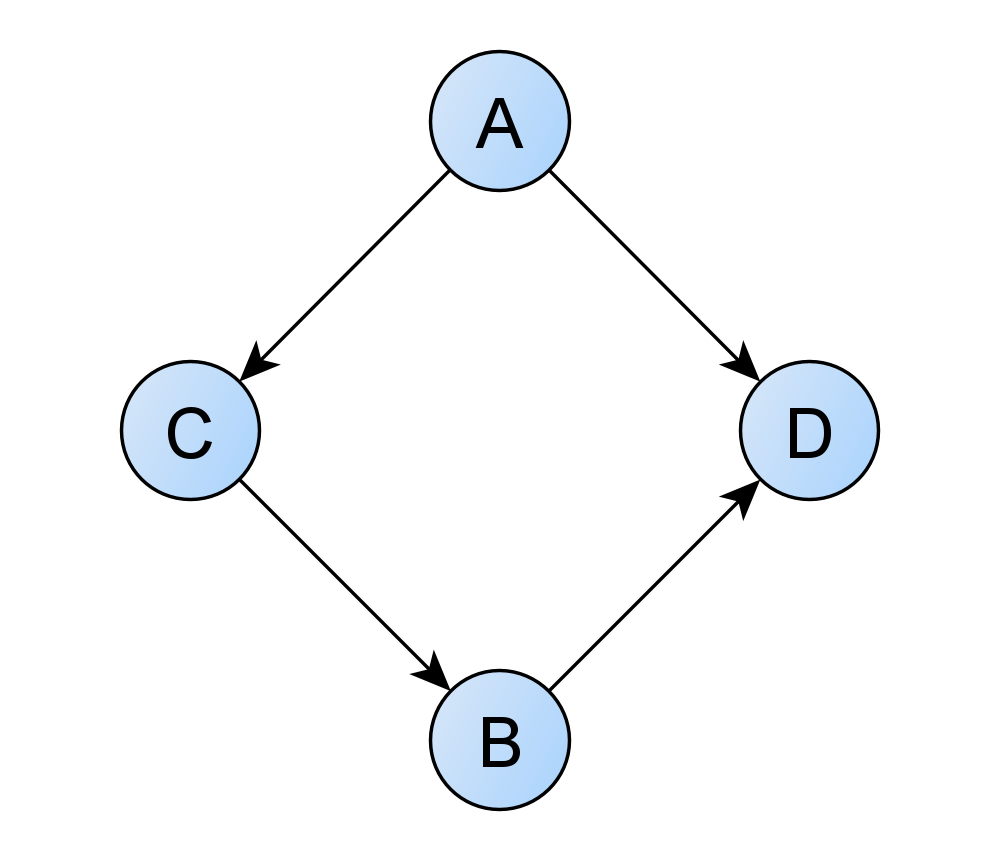
\includegraphics[width=7cm]{img/fermeture_transitive_0.png}}{7cm}

D'après la propriété précédente, étant donné que ce graphe possède 4 sommets on a $$\widehat{M}=M\oplus M^{[2]}\oplus M^{[3]}$$
En pratique, on calcule $M^2$, $M^3$ puis $M+M^2+M^3$ et on remplace chaque coefficient non nul par un 1.\\
Avec la calculatrice on obtient:
$M^2=\begin{pmatrix}0&1&0&0\\0&0&0&0\\0&0&0&1\\0&0&0&0\end{pmatrix}$ et 
$M^3=\begin{pmatrix}0&0&0&1\\0&0&0&0\\0&0&0&0\\0&0&0&0\end{pmatrix}$ de sorte que
$$M+M^2+M^3=\begin{pmatrix}0&1&1&2\\0&0&0&1\\0&1&0&1\\0&0&0&0\end{pmatrix}$$
Donc en définitive $\widehat{M}=\begin{pmatrix}0&1&1&1\\0&0&0&1\\0&1&0&1\\0&0&0&0\end{pmatrix}$
et on aboutit au graphe suivant :
\begin{center}
\includegraphics*[width=7cm]{img/fermeture_transitive_1.png}
\end{center}
où l'on a fait figurer en rouge les \og raccourcis\fg{} ajoutés. On peut remarquer que $M^3$ n'apporte pas grand-chose ici, car son seul coefficient non nul dit qu'il y a un chemin de longueur 3 : $(A,\,C,\,B,\,D)$ reliant $A$ et $D$, mais comme l'arc $(A,\,D)$ existe déjà, \og le raccourci est déjà là\fg{}.



\end{methode}
\end{document}
